\chapter{Extensión de la Base de Datos FER-2013 } \label{Chapter:6}

Obtenidos unos resultados más que aceptables y eficientes en lo que respecta al tiempo de entrenamiento, se ha intentado dar un paso más allá con la intención de mejorar las tasas de acierto y la calidad de la base de datos inicial mediante la implementación de una Red Generativa Antagónica de Ciclo Consecuente (CycleGAN) \cite{cycleGAN} que permita la producción artificial de imágenes y, por lo tanto, la eliminación del desequilibrio de la distribución de clases del conjunto FER-2013. En un principio tan sólo se pretende aumentar el número de datos etiquetados con la expresión facial de asco, que como se vio en la \autoref{Table:FER-2013} es con diferencia el gesto con menor representación. Las imágenes a partir de las cuales se pretenderá generar esta última emoción corresponderán, dada la adaptabilidad de su naturaleza, a la clase de la expresión neutral.

\section{Arquitectura propuesta}

La arquitectura aquí desarrollada y esquematizada en la \autoref{fig:cycleGAN} es una adaptación de la estructura propuesta en el documento original de las redes CycleGAN y que ha demostrado unos resultados más que razonables en el área de las redes generativas de base neuronal. Asimismo, al igual que los modelos descritos anteriormente, la implementación se ha llevada a cabo íntegramente en la API de Keras y sobre TensorFlow.

\subsection{Red generadora}

\begin{figure}
  \centering
  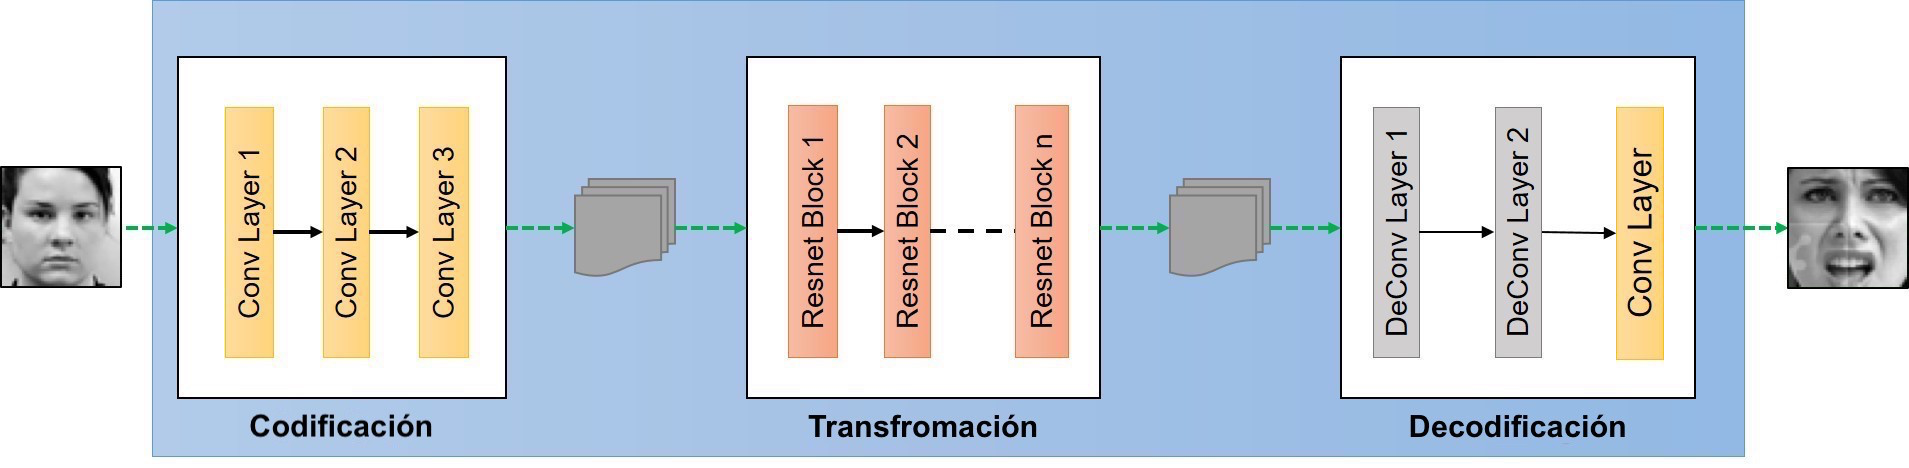
\includegraphics[width=\textwidth]{Images/Generator.png}
  \caption{Arquitectura simplificada del generador de la red CycleGAN \cite{img:CycleGAN}.}
  \label{fig:Generator}
\end{figure}

Desde un enfoque de alto nivel es posible dividir la red del generador en 3 módulos distintos dispuestos según la \autoref{fig:Generator}:
\begin{itemize}
    \item \textbf{Módulo de codificación}. Utiliza 3 capas convolucionales que extraen las características superficiales y disminuyen el mapa de activación de la imagen inyectada.
    \item \textbf{Módulo de transformación}. Está formado básicamente por 6 módulos residuales (\autoref{fig:ResNetBlock}) que utilizan filtros convolucionales de tamaño reducido ($3\times 3$) y que favorecen la estabilización de las respuestas de las redes profundas.
    \item \textbf{Módulo de decodificación}. Su función es exactamente la opuesta al primer módulo ya que es precisamente el que trata de reconstruir y trasladar la imagen original etiquetada con la emoción neutral al dominio objetivo que corresponde a la expresión de asco. Para tal fin se emplean dos capas deconvolucionales que recomponen el ancho y el alto de la imagen y una última capa convolucional que restaura los canales de la representación inicial.
\end{itemize}

Asimismo, cabe destacar que son utilizadas en cada una de las capas la función de activación ReLU y la normalización de instancias.

\subsection{Red discriminativa}

\begin{figure}
  \centering
  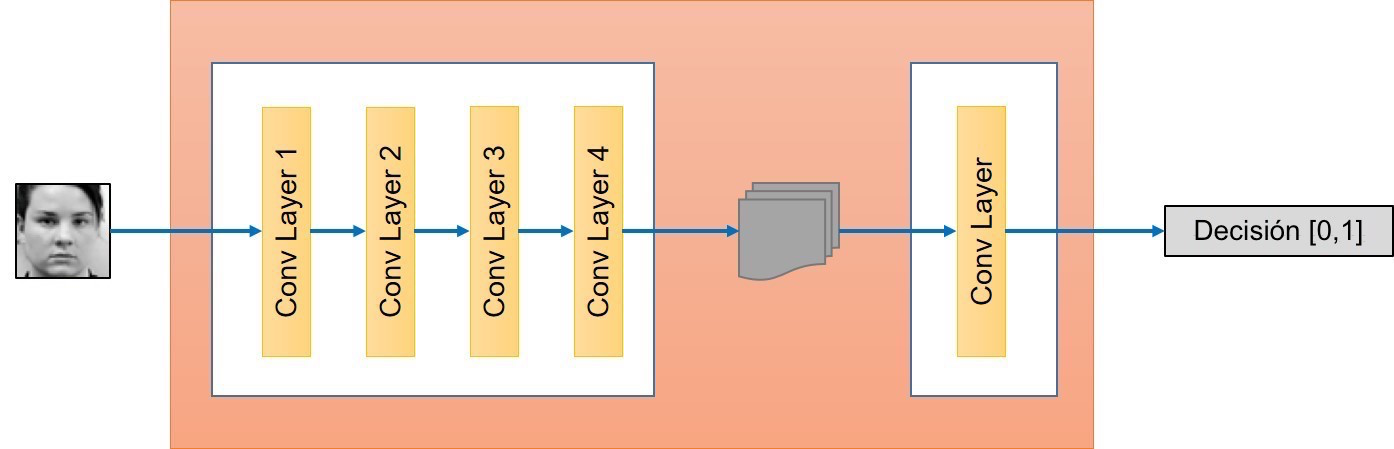
\includegraphics[width=\textwidth]{Images/Discriminator.png}
  \caption{Arquitectura simplificada del discriminador de la red CycleGAN \cite{img:CycleGAN}.}
  \label{fig:Discriminator}
\end{figure}

Presenta una estructura simple de 5 capas convolucionales de tamaño $4\times 4$ apiladas con una mínima alteración en el último nivel para permitir el cálculo de la función de pérdidas de mínimos cuadrados del discriminador y que consiste en la supresión de la función de activación y de la unidad de normalización de instancias final \cite{LSGAN}.

El parámetro de pendiente para la función de activación Leaky ReLU es 0.2


La arquitectura comprimida puede observarse en la \autoref{fig:Discriminator}.






\section{Entrenamiento}




\subsection{Preprocesamiento de los datos}



\subsection{Despliegue del modelo en la plataforma Google Cloud}




\section{Resultados}